\chapter{Concept of a Redundant HTN Planning Architecture}



\section{Technical Problem Definition}
% Input-process-output model -- include with % Input-process-output model -- include with % Input-process-output model -- include with \input{chapters/ipo_model}
% Needs only TikZ + the positioning library (already loaded via forest in main.tex)
\begin{figure}[H]
  \centering
  \begin{tikzpicture}[
      >=latex,
      font=\small,
      io/.style  ={draw, rounded corners=4pt, minimum width=2.6cm, minimum height=1.1cm},
      proc/.style={draw, fill=blue!6, minimum width=2.8cm, minimum height=1.1cm},
      note/.style={font=\scriptsize\itshape, text=black!60, align=center},
      flow/.style={->, thick},
    ]
    \node[io]                    (in)   {Input};
    \node[proc, right=1.6cm of in]  (proc) {Process};
    \node[io,   right=1.6cm of proc] (out)  {Output};

    % Side bars: flowchart symbol for a (predefined) process
    \draw ([xshift=4pt]proc.north west) -- ([xshift=4pt]proc.south west);
    \draw ([xshift=-4pt]proc.north east) -- ([xshift=-4pt]proc.south east);

    \draw[flow] (in)   -- (proc);
    \draw[flow] (proc) -- (out);

    % Example sources and sinks
    \node[note, below=3pt of in]  {e.g.\ sensors,\\sub-systems};
    \node[note, below=3pt of out] {e.g.\ actuators,\\sub-systems};
  \end{tikzpicture}

  \caption[Input--process--output model]{%
    Input--process--output model. The process receives its input from
    other systems such as sensors and passes its output on to further
    sub-systems such as actuators. As the only element between input and
    output, the process is a single point of failure (SPOF).}
  \label{fig:ipo-model}
\end{figure}

% Needs only TikZ + the positioning library (already loaded via forest in main.tex)
\begin{figure}[H]
  \centering
  \begin{tikzpicture}[
      >=latex,
      font=\small,
      io/.style  ={draw, rounded corners=4pt, minimum width=2.6cm, minimum height=1.1cm},
      proc/.style={draw, fill=blue!6, minimum width=2.8cm, minimum height=1.1cm},
      note/.style={font=\scriptsize\itshape, text=black!60, align=center},
      flow/.style={->, thick},
    ]
    \node[io]                    (in)   {Input};
    \node[proc, right=1.6cm of in]  (proc) {Process};
    \node[io,   right=1.6cm of proc] (out)  {Output};

    % Side bars: flowchart symbol for a (predefined) process
    \draw ([xshift=4pt]proc.north west) -- ([xshift=4pt]proc.south west);
    \draw ([xshift=-4pt]proc.north east) -- ([xshift=-4pt]proc.south east);

    \draw[flow] (in)   -- (proc);
    \draw[flow] (proc) -- (out);

    % Example sources and sinks
    \node[note, below=3pt of in]  {e.g.\ sensors,\\sub-systems};
    \node[note, below=3pt of out] {e.g.\ actuators,\\sub-systems};
  \end{tikzpicture}

  \caption[Input--process--output model]{%
    Input--process--output model. The process receives its input from
    other systems such as sensors and passes its output on to further
    sub-systems such as actuators. As the only element between input and
    output, the process is a single point of failure (SPOF).}
  \label{fig:ipo-model}
\end{figure}

% Needs only TikZ + the positioning library (already loaded via forest in main.tex)
\begin{figure}[H]
  \centering
  \begin{tikzpicture}[
      >=latex,
      font=\small,
      io/.style  ={draw, rounded corners=4pt, minimum width=2.6cm, minimum height=1.1cm},
      proc/.style={draw, fill=blue!6, minimum width=2.8cm, minimum height=1.1cm},
      note/.style={font=\scriptsize\itshape, text=black!60, align=center},
      flow/.style={->, thick},
    ]
    \node[io]                    (in)   {Input};
    \node[proc, right=1.6cm of in]  (proc) {Process};
    \node[io,   right=1.6cm of proc] (out)  {Output};

    % Side bars: flowchart symbol for a (predefined) process
    \draw ([xshift=4pt]proc.north west) -- ([xshift=4pt]proc.south west);
    \draw ([xshift=-4pt]proc.north east) -- ([xshift=-4pt]proc.south east);

    \draw[flow] (in)   -- (proc);
    \draw[flow] (proc) -- (out);

    % Example sources and sinks
    \node[note, below=3pt of in]  {e.g.\ sensors,\\sub-systems};
    \node[note, below=3pt of out] {e.g.\ actuators,\\sub-systems};
  \end{tikzpicture}

  \caption[Input--process--output model]{%
    Input--process--output model. The process receives its input from
    other systems such as sensors and passes its output on to further
    sub-systems such as actuators. As the only element between input and
    output, the process is a single point of failure (SPOF).}
  \label{fig:ipo-model}
\end{figure}


Using the model above, it is simpler to show what role TMR has as the process which mitigates a possible SPOF in a system view. Input would come from other systems, e.g. sensors, sub-systems, etc., and needs to be received by the process. The process then passes forward its output to other sub-systems, e.g. actuators.

The first question considers \textit{what} is actually to be solved for with the design and which aspects have been previously developed. This follows the principle in requirements engineering on the left side of the V-model and is a start for the problem and target definition.
Both coordination and communication in distributed computing have been extensively researched. \textcite{lamport_time_1978} laid the foundation for logical clocks, ``happened before'' relation, etc. Same can be said about lower level communication including but not limited to Remote Procedure Calls (RPC) and Remote Method Invocations (RMI) \parencite{steen_distributed_2025}. This shifts the focus of the problem from coordination and communication which is relevant to the foundational concepts of distributed computing, to the question of how coordination and communication need to be designed for a redundantly designed HTN. Here it is necessary to specify which target the redundant design needs to fulfill, which allows the derivation of the functional logic of coordination. The target serves as the system-level goal while the coordination is a means to said goal. Generally in a distributed system (especially complex ones), there are many different failures that are possible \parencite{maurya_reliability_2020}. Hence it is necessary to define which type of failure will be analyzed here.
For this writing, the target of the system is defined to mitigate the failure of a node in the TMR cluster by restarting the affected node. A top-down approach will be used to define which states are used by the system, what functional logic they perform and which components realize the functions necessary.

\section{Assumptions and Scope}

The previous chapters introduced the concepts relevant to this thesis: HTN planning and redundancy through replication. This chapter combines them into an architecture concept for a redundant planning cluster. Before the concept is developed, the following section defines which of these concepts it builds on and what assumptions it makes, as these determine the conditions under which the architecture is valid.

DFS is a deterministic search algorithm in good agreement with behavior per-node in a cluster of redundant nodes which run a HTN with SHOP. The reproducibility of both a deterministic process and outcome allow for a diagnosis or determination of an error when either differ from their expected behavior at runtime. This is beneficial to the design process as expected behavior can be defined offline and compared against observed behavior at runtime, so failures and recovery can be specified in advance during development.

While determinism ensures consistent behavior within each node, the cluster as a whole must also be predictable. In a statically configured system, the set of relevant data, participants and information are fixed and known. This means for network behavior and topology that a static cluster will be considered because it allows for full offline definition of the cluster at time of design and development for any mechanisms which TMR and HTN require.

Connecting this to the topic of communication within the nodes is the possibility of errors in either transmission medium or the message itself even at successful delivery at the recipient. While message delivery is defined as guaranteed between sender and recipient, it is still possible that errors occur on a bit-level due to electromagnetic variance or hardware problems in electronic components, e.g. CPU, RAM, a bus system or other which aren't a fault of the actual transmission itself. The guarantee for message delivery is assumed based on the existing standards for avionic buses, e.g. MIL-STD-1553 \parencite{milstd1553c} which defines mechanisms for retransmission and bit-level correction like parity bits, Manchester II, etc.

The next design decision concerns the type of redundancy considered. Triple modular redundancy will be used as it's a foundational concept used widely in many safety-critical domains including but not limited to avionic, automotive, medical systems as stated earlier. The goal of the design concept is to enable fault-tolerance and resilience. The last part currently excluded for concept development are advanced architectures \parencite{bonna_triple_2019, anwer_dynamic_2020, hamilton_adaptive-hybrid_2019} which make use of TMR as one component of the redundancy model. Focus will instead be put on concepts from these architectures to a more basic model.

% Define the scope, assumptions, requirements, and use case.

As a method of work, some principles from systems engineering will be used to serve as a framework to guide the process to find a solution concept. The main focus of systems engineering is to focus on the system as a whole. It is relevant to consider which interactions take place both with external systems as well as internally in the system of interest. Other external factors are the customer's (or user's) needs, interfaces, capabilities of the system for the user and more which must be included in a system's design. One approach of systems engineering is the V-Modell which encompasses many steps from the definition of requirements to high-level design, detailed design and on the right side system verification and validation. The stages on the left side will also be used here as a reference. \parencite{kossiakoff_systems_2020}

Because the scope is focused on concept development and prototyping, the left side of the V-model will be used here as a guide to first define the system level goal, the system's design and functions which must be assigned to the components to be implemented. At the end, a simple proof of concept will be used to demonstrate an implementation that can be used as an example.

% V-model -- include with % V-model -- include with % V-model -- include with \input{chapters/vmodel}
% Needs only TikZ + the positioning library (already loaded via forest in main.tex)
\begin{figure}[H]
  \centering
  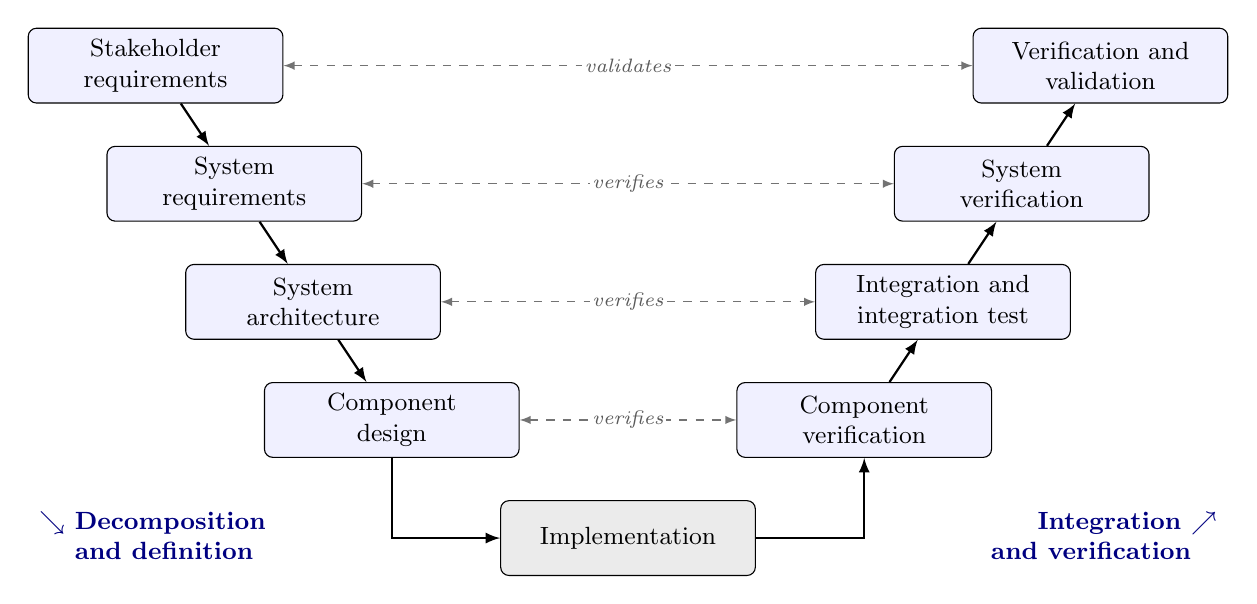
\begin{tikzpicture}[
      >=latex,
      font=\small,
      phase/.style={draw, rounded corners=3pt, fill=blue!6, align=center,
                    minimum width=3.2cm, minimum height=0.95cm, text width=3.0cm},
      impl/.style ={phase, fill=black!8},
      flow/.style ={->, thick},
      link/.style ={<->, dashed, black!55},
      lbl/.style  ={font=\scriptsize\itshape, text=black!65, fill=white, inner sep=1pt},
    ]
    % Left branch: specification and design (top to bottom)
    \node[phase] (req)  at (0.0, 0.0)  {Stakeholder\\requirements};
    \node[phase] (sys)  at (1.0,-1.5)  {System\\requirements};
    \node[phase] (arch) at (2.0,-3.0)  {System\\architecture};
    \node[phase] (comp) at (3.0,-4.5)  {Component\\design};

    % Bottom
    \node[impl]  (impl) at (6.0,-6.0)  {Implementation};

    % Right branch: integration and verification (bottom to top)
    \node[phase] (cver) at (9.0,-4.5)  {Component\\verification};
    \node[phase] (int)  at (10.0,-3.0) {Integration and\\integration test};
    \node[phase] (sver) at (11.0,-1.5) {System\\verification};
    \node[phase] (val)  at (12.0, 0.0) {Verification and\\validation};

    % Process flow along the V
    \draw[flow] (req)  -- (sys);
    \draw[flow] (sys)  -- (arch);
    \draw[flow] (arch) -- (comp);
    \draw[flow] (comp) |- (impl);
    \draw[flow] (impl) -| (cver);
    \draw[flow] (cver) -- (int);
    \draw[flow] (int)  -- (sver);
    \draw[flow] (sver) -- (val);

    % Verification / validation relationships across the V
    \draw[link] (req.east)  -- node[lbl] {validates} (val.west);
    \draw[link] (sys.east)  -- node[lbl] {verifies}  (sver.west);
    \draw[link] (arch.east) -- node[lbl] {verifies}  (int.west);
    \draw[link] (comp.east) -- node[lbl] {verifies}  (cver.west);

    % Branch labels (bottom corners, outside the V)
    \node[font=\small\bfseries, text=blue!50!black, align=left, anchor=west]
      at (-1.6,-6.0) {$\searrow$ Decomposition\\\phantom{$\searrow$} and definition};
    \node[font=\small\bfseries, text=blue!50!black, align=right, anchor=east]
      at (13.6,-6.0) {Integration $\nearrow$\\and verification\phantom{$\nearrow$}};
  \end{tikzpicture}

  \caption[V-model of the system development process]{%
    V-model of the system development process. The left branch decomposes
    stakeholder requirements step by step into system requirements, an
    architecture and component designs; after implementation, the right
    branch integrates the components into the complete system. Each
    level on the right is verified against its counterpart on the left
    (dashed arrows), and the finished system is validated against the
    original stakeholder requirements.}
  \label{fig:vmodel}
\end{figure}

% Needs only TikZ + the positioning library (already loaded via forest in main.tex)
\begin{figure}[H]
  \centering
  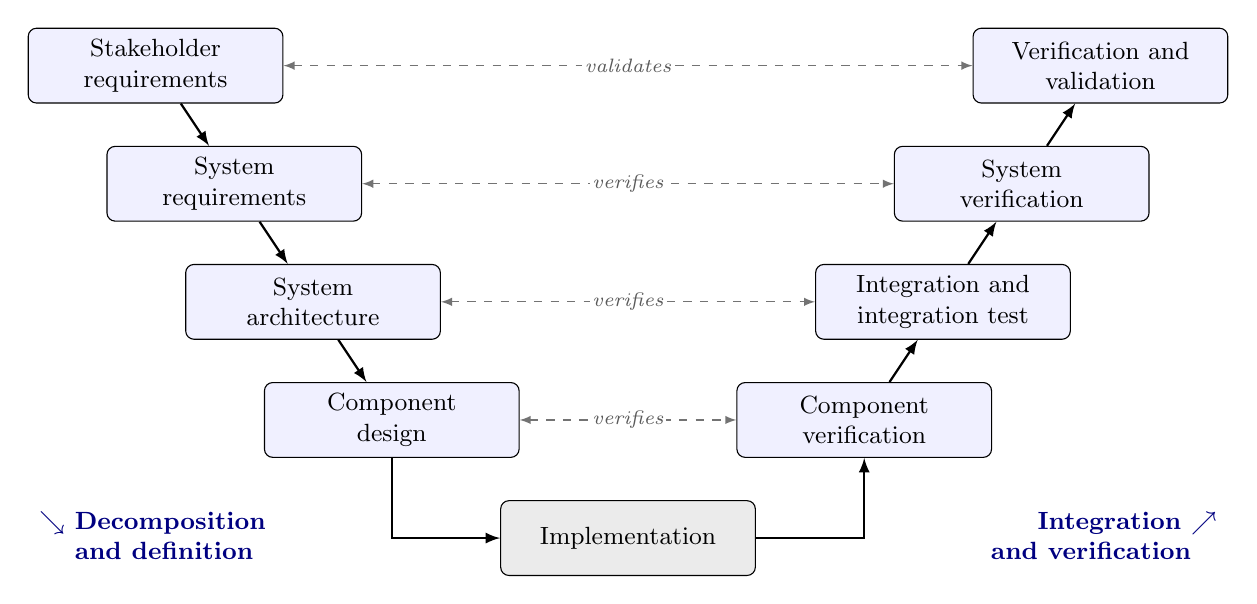
\begin{tikzpicture}[
      >=latex,
      font=\small,
      phase/.style={draw, rounded corners=3pt, fill=blue!6, align=center,
                    minimum width=3.2cm, minimum height=0.95cm, text width=3.0cm},
      impl/.style ={phase, fill=black!8},
      flow/.style ={->, thick},
      link/.style ={<->, dashed, black!55},
      lbl/.style  ={font=\scriptsize\itshape, text=black!65, fill=white, inner sep=1pt},
    ]
    % Left branch: specification and design (top to bottom)
    \node[phase] (req)  at (0.0, 0.0)  {Stakeholder\\requirements};
    \node[phase] (sys)  at (1.0,-1.5)  {System\\requirements};
    \node[phase] (arch) at (2.0,-3.0)  {System\\architecture};
    \node[phase] (comp) at (3.0,-4.5)  {Component\\design};

    % Bottom
    \node[impl]  (impl) at (6.0,-6.0)  {Implementation};

    % Right branch: integration and verification (bottom to top)
    \node[phase] (cver) at (9.0,-4.5)  {Component\\verification};
    \node[phase] (int)  at (10.0,-3.0) {Integration and\\integration test};
    \node[phase] (sver) at (11.0,-1.5) {System\\verification};
    \node[phase] (val)  at (12.0, 0.0) {Verification and\\validation};

    % Process flow along the V
    \draw[flow] (req)  -- (sys);
    \draw[flow] (sys)  -- (arch);
    \draw[flow] (arch) -- (comp);
    \draw[flow] (comp) |- (impl);
    \draw[flow] (impl) -| (cver);
    \draw[flow] (cver) -- (int);
    \draw[flow] (int)  -- (sver);
    \draw[flow] (sver) -- (val);

    % Verification / validation relationships across the V
    \draw[link] (req.east)  -- node[lbl] {validates} (val.west);
    \draw[link] (sys.east)  -- node[lbl] {verifies}  (sver.west);
    \draw[link] (arch.east) -- node[lbl] {verifies}  (int.west);
    \draw[link] (comp.east) -- node[lbl] {verifies}  (cver.west);

    % Branch labels (bottom corners, outside the V)
    \node[font=\small\bfseries, text=blue!50!black, align=left, anchor=west]
      at (-1.6,-6.0) {$\searrow$ Decomposition\\\phantom{$\searrow$} and definition};
    \node[font=\small\bfseries, text=blue!50!black, align=right, anchor=east]
      at (13.6,-6.0) {Integration $\nearrow$\\and verification\phantom{$\nearrow$}};
  \end{tikzpicture}

  \caption[V-model of the system development process]{%
    V-model of the system development process. The left branch decomposes
    stakeholder requirements step by step into system requirements, an
    architecture and component designs; after implementation, the right
    branch integrates the components into the complete system. Each
    level on the right is verified against its counterpart on the left
    (dashed arrows), and the finished system is validated against the
    original stakeholder requirements.}
  \label{fig:vmodel}
\end{figure}

% Needs only TikZ + the positioning library (already loaded via forest in main.tex)
\begin{figure}[H]
  \centering
  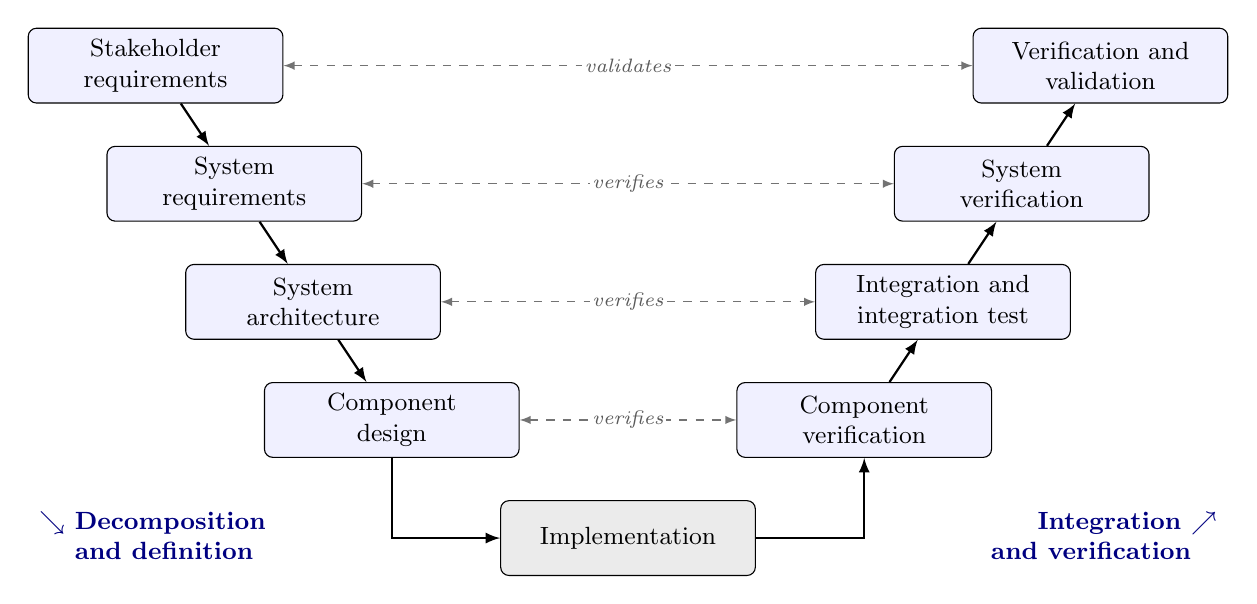
\begin{tikzpicture}[
      >=latex,
      font=\small,
      phase/.style={draw, rounded corners=3pt, fill=blue!6, align=center,
                    minimum width=3.2cm, minimum height=0.95cm, text width=3.0cm},
      impl/.style ={phase, fill=black!8},
      flow/.style ={->, thick},
      link/.style ={<->, dashed, black!55},
      lbl/.style  ={font=\scriptsize\itshape, text=black!65, fill=white, inner sep=1pt},
    ]
    % Left branch: specification and design (top to bottom)
    \node[phase] (req)  at (0.0, 0.0)  {Stakeholder\\requirements};
    \node[phase] (sys)  at (1.0,-1.5)  {System\\requirements};
    \node[phase] (arch) at (2.0,-3.0)  {System\\architecture};
    \node[phase] (comp) at (3.0,-4.5)  {Component\\design};

    % Bottom
    \node[impl]  (impl) at (6.0,-6.0)  {Implementation};

    % Right branch: integration and verification (bottom to top)
    \node[phase] (cver) at (9.0,-4.5)  {Component\\verification};
    \node[phase] (int)  at (10.0,-3.0) {Integration and\\integration test};
    \node[phase] (sver) at (11.0,-1.5) {System\\verification};
    \node[phase] (val)  at (12.0, 0.0) {Verification and\\validation};

    % Process flow along the V
    \draw[flow] (req)  -- (sys);
    \draw[flow] (sys)  -- (arch);
    \draw[flow] (arch) -- (comp);
    \draw[flow] (comp) |- (impl);
    \draw[flow] (impl) -| (cver);
    \draw[flow] (cver) -- (int);
    \draw[flow] (int)  -- (sver);
    \draw[flow] (sver) -- (val);

    % Verification / validation relationships across the V
    \draw[link] (req.east)  -- node[lbl] {validates} (val.west);
    \draw[link] (sys.east)  -- node[lbl] {verifies}  (sver.west);
    \draw[link] (arch.east) -- node[lbl] {verifies}  (int.west);
    \draw[link] (comp.east) -- node[lbl] {verifies}  (cver.west);

    % Branch labels (bottom corners, outside the V)
    \node[font=\small\bfseries, text=blue!50!black, align=left, anchor=west]
      at (-1.6,-6.0) {$\searrow$ Decomposition\\\phantom{$\searrow$} and definition};
    \node[font=\small\bfseries, text=blue!50!black, align=right, anchor=east]
      at (13.6,-6.0) {Integration $\nearrow$\\and verification\phantom{$\nearrow$}};
  \end{tikzpicture}

  \caption[V-model of the system development process]{%
    V-model of the system development process. The left branch decomposes
    stakeholder requirements step by step into system requirements, an
    architecture and component designs; after implementation, the right
    branch integrates the components into the complete system. Each
    level on the right is verified against its counterpart on the left
    (dashed arrows), and the finished system is validated against the
    original stakeholder requirements.}
  \label{fig:vmodel}
\end{figure}


% Describe the proposed architecture and design decisions.

\section{System States}

As an initial approach, it is useful to consider what is generally required for a TMR node cluster before specifying it further to a HTN. Firstly, it is to be defined what an expected normal mode of operation must fulfill and which functionality it performs. The second mode of operation is the response to a failure that has occurred during normal operation. In any distributed system, this requires state synchronization in the system. Dependent on the type of synchronization that is used in the system \parencite{viotti_consistency_2017}, it needs to be defined which components must be synchronized and in what manner. This will be defined later in component definition. As a start, three system states will be defined: Active, Failure and Standby.

Active is the expected system behavior during normal operation where input data is received, passed to HTN worker nodes, a result is determined and forwarded as output. The third system state is Standby which would be during system recovery where all other components must wait until normal operation may resume, upon which the system transitions again to Active state.

% Node state machine (UML style) -- include with % Node state machine (UML style) -- include with % Node state machine (UML style) -- include with \input{chapters/node_states}
% Needs only TikZ + the positioning library (already loaded via forest in main.tex)
\begin{figure}[H]
  \centering
  \begin{tikzpicture}[
      >=latex,
      font=\small,
      state/.style ={draw, thick, rounded corners=8pt, fill=blue!6,
                     minimum width=2.8cm, minimum height=1.0cm},
      fail/.style  ={state, fill=red!8, draw=red!60!black},
      init/.style  ={circle, fill=black, inner sep=0pt, minimum size=9pt},
      final/.style ={circle, draw, thick, inner sep=0pt, minimum size=13pt,
                     path picture={\fill (path picture bounding box.center) circle (3.5pt);}},
      trans/.style ={->, thick},
      lbl/.style   ={font=\scriptsize\itshape, text=black!70},
    ]
    % States
    \node[state]                       (act)  {Active};
    \node[init,  above=1.3cm of act]   (ini)  {};
    \node[final, left=2.6cm of act]    (fin)  {};
    \node[state, right=3.4cm of act]   (stb)  {Standby};
    \node[fail,  below=1.8cm of act]   (flt)  {Failure};

    % Transitions
    \draw[trans] (ini) -- node[lbl, right] {start-up} (act);
    \draw[trans] (act) -- node[lbl, above] {mission end} (fin);
    \draw[trans] (act) -- node[lbl, right] {fault detected} (flt);
    \draw[trans] (flt) -| node[lbl, below, pos=0.25] {recovered} (stb);
    \draw[trans] (stb) -- node[lbl, above] {reintegrated} (act);
  \end{tikzpicture}

  \caption[State machine of a redundant node]{%
    State machine of a redundant node. After start-up the node is
    \emph{Active}. When a fault is detected it enters \emph{Failure} and is
    excluded from the redundancy set. Once recovered it waits in
    \emph{Standby} until it is reintegrated as an active node. The node
    leaves the state machine when the mission ends.}
  \label{fig:node-states}
\end{figure}

% Needs only TikZ + the positioning library (already loaded via forest in main.tex)
\begin{figure}[H]
  \centering
  \begin{tikzpicture}[
      >=latex,
      font=\small,
      state/.style ={draw, thick, rounded corners=8pt, fill=blue!6,
                     minimum width=2.8cm, minimum height=1.0cm},
      fail/.style  ={state, fill=red!8, draw=red!60!black},
      init/.style  ={circle, fill=black, inner sep=0pt, minimum size=9pt},
      final/.style ={circle, draw, thick, inner sep=0pt, minimum size=13pt,
                     path picture={\fill (path picture bounding box.center) circle (3.5pt);}},
      trans/.style ={->, thick},
      lbl/.style   ={font=\scriptsize\itshape, text=black!70},
    ]
    % States
    \node[state]                       (act)  {Active};
    \node[init,  above=1.3cm of act]   (ini)  {};
    \node[final, left=2.6cm of act]    (fin)  {};
    \node[state, right=3.4cm of act]   (stb)  {Standby};
    \node[fail,  below=1.8cm of act]   (flt)  {Failure};

    % Transitions
    \draw[trans] (ini) -- node[lbl, right] {start-up} (act);
    \draw[trans] (act) -- node[lbl, above] {mission end} (fin);
    \draw[trans] (act) -- node[lbl, right] {fault detected} (flt);
    \draw[trans] (flt) -| node[lbl, below, pos=0.25] {recovered} (stb);
    \draw[trans] (stb) -- node[lbl, above] {reintegrated} (act);
  \end{tikzpicture}

  \caption[State machine of a redundant node]{%
    State machine of a redundant node. After start-up the node is
    \emph{Active}. When a fault is detected it enters \emph{Failure} and is
    excluded from the redundancy set. Once recovered it waits in
    \emph{Standby} until it is reintegrated as an active node. The node
    leaves the state machine when the mission ends.}
  \label{fig:node-states}
\end{figure}

% Needs only TikZ + the positioning library (already loaded via forest in main.tex)
\begin{figure}[H]
  \centering
  \begin{tikzpicture}[
      >=latex,
      font=\small,
      state/.style ={draw, thick, rounded corners=8pt, fill=blue!6,
                     minimum width=2.8cm, minimum height=1.0cm},
      fail/.style  ={state, fill=red!8, draw=red!60!black},
      init/.style  ={circle, fill=black, inner sep=0pt, minimum size=9pt},
      final/.style ={circle, draw, thick, inner sep=0pt, minimum size=13pt,
                     path picture={\fill (path picture bounding box.center) circle (3.5pt);}},
      trans/.style ={->, thick},
      lbl/.style   ={font=\scriptsize\itshape, text=black!70},
    ]
    % States
    \node[state]                       (act)  {Active};
    \node[init,  above=1.3cm of act]   (ini)  {};
    \node[final, left=2.6cm of act]    (fin)  {};
    \node[state, right=3.4cm of act]   (stb)  {Standby};
    \node[fail,  below=1.8cm of act]   (flt)  {Failure};

    % Transitions
    \draw[trans] (ini) -- node[lbl, right] {start-up} (act);
    \draw[trans] (act) -- node[lbl, above] {mission end} (fin);
    \draw[trans] (act) -- node[lbl, right] {fault detected} (flt);
    \draw[trans] (flt) -| node[lbl, below, pos=0.25] {recovered} (stb);
    \draw[trans] (stb) -- node[lbl, above] {reintegrated} (act);
  \end{tikzpicture}

  \caption[State machine of a redundant node]{%
    State machine of a redundant node. After start-up the node is
    \emph{Active}. When a fault is detected it enters \emph{Failure} and is
    excluded from the redundancy set. Once recovered it waits in
    \emph{Standby} until it is reintegrated as an active node. The node
    leaves the state machine when the mission ends.}
  \label{fig:node-states}
\end{figure}


\section{Functional Logic}

For functional logic, the basis for TMR is to use a voter to mask faults. One principle found in best practices can be applied here by providing each component only with the necessary information that it requires for the functions it is defined for. This connects later to the next part: common interfaces and exchange of information between components.

In Active state, synchronization is needed at different points during normal operation.
Input data may be received from different sources at varying times and potential delays are also involved. Therefore a synchronization point \(sync1\) is defined at the start of the process. The worker nodes themselves may have different execution times until completion of their task. This is the second synchronization point \(sync2\). Then before the output data can be sent forward, a third synchronization point \(sync3\) is required from TMR voter resolution to the decision of how the voter result is to be used.

% TMR voting cycle (UML activity diagram) -- include with % TMR voting cycle (UML activity diagram) -- include with % TMR voting cycle (UML activity diagram) -- include with \input{chapters/voting_cycle}
% Needs only TikZ + the positioning library (already loaded via forest in main.tex)
\begin{figure}[H]
  \centering
  \begin{tikzpicture}[
      >=latex,
      font=\small,
      action/.style ={draw, thick, rounded corners=6pt, fill=blue!6, align=center,
                      minimum width=2.4cm, minimum height=1.1cm},
      init/.style   ={circle, fill=black, inner sep=0pt, minimum size=9pt},
      final/.style  ={circle, draw, thick, inner sep=0pt, minimum size=13pt,
                      path picture={\fill (path picture bounding box.center) circle (3.5pt);}},
      decision/.style={diamond, draw, thick, aspect=1, inner sep=0pt, minimum size=0.9cm},
      bar/.style    ={fill=black, minimum width=4pt, minimum height=2.2cm, inner sep=0pt},
      flow/.style   ={->, thick},
      sync/.style   ={dashed, black!55},
      synclbl/.style={font=\small, text=black!70},
    ]
    % Nodes
    \node[init]     (ini) at (0,0)     {};
    \node[bar]      (bar) at (2.3,0)   {};
    \node[action]   (wrk) at (5.1,0)   {Worker nodes\\process};
    \node[action]   (vot) at (9.0,0)   {Voter resolution};
    \node[decision] (dec) at (12.5,0)  {};
    \node[final]    (fin) at (14.3,0)  {};
    \node[action, fill=red!8] (oth) at (12.5,-2.8) {Discard result};
    \node[final]    (fin2) at (14.3,-2.8) {};

    \node[font=\small, align=center, above=3pt of dec] {Use vote\\result};

    % Input data distributed to the worker nodes
    \coordinate (split) at (1.0,0);
    \draw[thick] (ini) -- (split);
    \draw[flow] (split) |- ([yshift= 0.7cm]bar.west);
    \draw[flow] (split) --  (bar.west);
    \draw[flow] (split) |- ([yshift=-0.7cm]bar.west);
    \node[font=\small, below=0.85cm of split, anchor=north] {input data};

    % Main flow
    \draw[flow] (bar) -- (wrk);
    \draw[flow] (wrk) -- (vot);
    \draw[flow] (vot) -- (dec);
    \draw[flow] (dec) -- node[above] {yes} (fin);
    \draw[flow] (dec) -- node[right] {no} (oth);
    \draw[flow] (oth) -- (fin2);

    % Synchronisation points
    \foreach \x/\name in {3.15/sync1, 7.05/sync2, 11.0/sync3} {
      \draw[sync] (\x, 1.5) -- (\x,-1.5);
      \node[synclbl, below] at (\x,-1.5) {\name};
    }
  \end{tikzpicture}

  \caption[Activity diagram of one TMR voting cycle]{%
    Activity diagram of one TMR voting cycle. The input data is
    distributed to all worker nodes, which process it in parallel; their
    results are passed to the voter. If the vote result can be used, the
    cycle ends with that result; otherwise the result is discarded. The dashed
    lines \emph{sync1}--\emph{sync3} mark the synchronization points
    between the stages.}
  \label{fig:voting-cycle}
\end{figure}

% Needs only TikZ + the positioning library (already loaded via forest in main.tex)
\begin{figure}[H]
  \centering
  \begin{tikzpicture}[
      >=latex,
      font=\small,
      action/.style ={draw, thick, rounded corners=6pt, fill=blue!6, align=center,
                      minimum width=2.4cm, minimum height=1.1cm},
      init/.style   ={circle, fill=black, inner sep=0pt, minimum size=9pt},
      final/.style  ={circle, draw, thick, inner sep=0pt, minimum size=13pt,
                      path picture={\fill (path picture bounding box.center) circle (3.5pt);}},
      decision/.style={diamond, draw, thick, aspect=1, inner sep=0pt, minimum size=0.9cm},
      bar/.style    ={fill=black, minimum width=4pt, minimum height=2.2cm, inner sep=0pt},
      flow/.style   ={->, thick},
      sync/.style   ={dashed, black!55},
      synclbl/.style={font=\small, text=black!70},
    ]
    % Nodes
    \node[init]     (ini) at (0,0)     {};
    \node[bar]      (bar) at (2.3,0)   {};
    \node[action]   (wrk) at (5.1,0)   {Worker nodes\\process};
    \node[action]   (vot) at (9.0,0)   {Voter resolution};
    \node[decision] (dec) at (12.5,0)  {};
    \node[final]    (fin) at (14.3,0)  {};
    \node[action, fill=red!8] (oth) at (12.5,-2.8) {Discard result};
    \node[final]    (fin2) at (14.3,-2.8) {};

    \node[font=\small, align=center, above=3pt of dec] {Use vote\\result};

    % Input data distributed to the worker nodes
    \coordinate (split) at (1.0,0);
    \draw[thick] (ini) -- (split);
    \draw[flow] (split) |- ([yshift= 0.7cm]bar.west);
    \draw[flow] (split) --  (bar.west);
    \draw[flow] (split) |- ([yshift=-0.7cm]bar.west);
    \node[font=\small, below=0.85cm of split, anchor=north] {input data};

    % Main flow
    \draw[flow] (bar) -- (wrk);
    \draw[flow] (wrk) -- (vot);
    \draw[flow] (vot) -- (dec);
    \draw[flow] (dec) -- node[above] {yes} (fin);
    \draw[flow] (dec) -- node[right] {no} (oth);
    \draw[flow] (oth) -- (fin2);

    % Synchronisation points
    \foreach \x/\name in {3.15/sync1, 7.05/sync2, 11.0/sync3} {
      \draw[sync] (\x, 1.5) -- (\x,-1.5);
      \node[synclbl, below] at (\x,-1.5) {\name};
    }
  \end{tikzpicture}

  \caption[Activity diagram of one TMR voting cycle]{%
    Activity diagram of one TMR voting cycle. The input data is
    distributed to all worker nodes, which process it in parallel; their
    results are passed to the voter. If the vote result can be used, the
    cycle ends with that result; otherwise the result is discarded. The dashed
    lines \emph{sync1}--\emph{sync3} mark the synchronization points
    between the stages.}
  \label{fig:voting-cycle}
\end{figure}

% Needs only TikZ + the positioning library (already loaded via forest in main.tex)
\begin{figure}[H]
  \centering
  \begin{tikzpicture}[
      >=latex,
      font=\small,
      action/.style ={draw, thick, rounded corners=6pt, fill=blue!6, align=center,
                      minimum width=2.4cm, minimum height=1.1cm},
      init/.style   ={circle, fill=black, inner sep=0pt, minimum size=9pt},
      final/.style  ={circle, draw, thick, inner sep=0pt, minimum size=13pt,
                      path picture={\fill (path picture bounding box.center) circle (3.5pt);}},
      decision/.style={diamond, draw, thick, aspect=1, inner sep=0pt, minimum size=0.9cm},
      bar/.style    ={fill=black, minimum width=4pt, minimum height=2.2cm, inner sep=0pt},
      flow/.style   ={->, thick},
      sync/.style   ={dashed, black!55},
      synclbl/.style={font=\small, text=black!70},
    ]
    % Nodes
    \node[init]     (ini) at (0,0)     {};
    \node[bar]      (bar) at (2.3,0)   {};
    \node[action]   (wrk) at (5.1,0)   {Worker nodes\\process};
    \node[action]   (vot) at (9.0,0)   {Voter resolution};
    \node[decision] (dec) at (12.5,0)  {};
    \node[final]    (fin) at (14.3,0)  {};
    \node[action, fill=red!8] (oth) at (12.5,-2.8) {Discard result};
    \node[final]    (fin2) at (14.3,-2.8) {};

    \node[font=\small, align=center, above=3pt of dec] {Use vote\\result};

    % Input data distributed to the worker nodes
    \coordinate (split) at (1.0,0);
    \draw[thick] (ini) -- (split);
    \draw[flow] (split) |- ([yshift= 0.7cm]bar.west);
    \draw[flow] (split) --  (bar.west);
    \draw[flow] (split) |- ([yshift=-0.7cm]bar.west);
    \node[font=\small, below=0.85cm of split, anchor=north] {input data};

    % Main flow
    \draw[flow] (bar) -- (wrk);
    \draw[flow] (wrk) -- (vot);
    \draw[flow] (vot) -- (dec);
    \draw[flow] (dec) -- node[above] {yes} (fin);
    \draw[flow] (dec) -- node[right] {no} (oth);
    \draw[flow] (oth) -- (fin2);

    % Synchronisation points
    \foreach \x/\name in {3.15/sync1, 7.05/sync2, 11.0/sync3} {
      \draw[sync] (\x, 1.5) -- (\x,-1.5);
      \node[synclbl, below] at (\x,-1.5) {\name};
    }
  \end{tikzpicture}

  \caption[Activity diagram of one TMR voting cycle]{%
    Activity diagram of one TMR voting cycle. The input data is
    distributed to all worker nodes, which process it in parallel; their
    results are passed to the voter. If the vote result can be used, the
    cycle ends with that result; otherwise the result is discarded. The dashed
    lines \emph{sync1}--\emph{sync3} mark the synchronization points
    between the stages.}
  \label{fig:voting-cycle}
\end{figure}


The reason for a rejection of the voted result is one common flaw with voter resolution. If a majority of the worker nodes' results is equally incorrect, the voter would resolve it as a valid result. This is a common mode failure (CMF) and is defined by \textcite{hodson_failure-tolerant_2024} as a failure that occurs due to a single event, design defect or violation of other independence assumptions. \textcite{mitra_common-mode_2000} describe several techniques to handle common mode failure, one aspect is to include methods that avoid CMF in the design and development process. It is important to mention here that any technique can only mitigate or reduce the effects of a CMF significantly, but cannot remove one entirely.

Following the principle of mitigating CMF in the design process, one choice will be proposed here by introduction of a rule set. A basic rule set can be defined following the logic of how SHOP works. Because tasks are ordered into their sequence of execution, a check can be defined per pair of any subsequent tasks A and B. If B is allowed to follow after A, then a 'pass' is determined. In the case of a task A before B, where B must not follow after A, a 'fail' is determined.

% Rule-set check of the voter result (UML activity diagram)
% include with % Rule-set check of the voter result (UML activity diagram)
% include with % Rule-set check of the voter result (UML activity diagram)
% include with \input{chapters/rule_check}
% Needs only TikZ + the positioning library (already loaded via forest in main.tex)
\begin{figure}[H]
  \centering
  \begin{tikzpicture}[
      >=latex,
      font=\small,
      action/.style  ={draw, thick, rounded corners=6pt, fill=blue!6, align=center,
                       minimum width=3.4cm, minimum height=0.95cm},
      good/.style    ={action, fill=green!8},
      bad/.style     ={action, fill=red!8},
      init/.style    ={circle, fill=black, inner sep=0pt, minimum size=9pt},
      final/.style   ={circle, draw, thick, inner sep=0pt, minimum size=13pt,
                       path picture={\fill (path picture bounding box.center) circle (3.5pt);}},
      decision/.style={diamond, draw, thick, aspect=1, inner sep=0pt, minimum size=0.9cm},
      flow/.style    ={->, thick},
    ]
    % Nodes
    \node[init]     (ini)  at (0, 0.0)  {};
    \node[action]   (res)  at (0,-1.2)  {Voter result\\(task sequence)};
    \node[action]   (pair) at (0,-2.7)  {Take next pair of\\subsequent tasks $(A, B)$};
    \node[decision] (d1)   at (0,-4.3)  {};
    \node[decision] (d2)   at (0,-5.9)  {};
    \node[good]     (pass) at (0,-7.4)  {Pass:\\use result};
    \node[final]    (f1)   at (0,-8.6)  {};
    \node[bad]      (fail) at (4.2,-4.3) {Fail: discard result,\\HTN calculates next task};
    \node[final]    (f2)   at (4.2,-5.6) {};

    % Decision labels
    \node[font=\small, anchor=south west] at ([xshift=5pt, yshift=2pt]d1.north)
      {Rule set allows $A$ before $B$?};
    \node[font=\small, anchor=west] at ([xshift=4pt]d2.east) {All pairs checked?};

    % Flow
    \draw[flow] (ini)  -- (res);
    \draw[flow] (res)  -- (pair);
    \draw[flow] (pair) -- (d1);
    \draw[flow] (d1) -- node[above] {no} (fail);
    \draw[flow] (fail) -- (f2);
    \draw[flow] (d1) -- node[right] {yes} (d2);
    \draw[flow] (d2) -- node[right] {yes} (pass);
    \draw[flow] (pass) -- (f1);
    % Loop back for the next pair
    \draw[flow] (d2.west) -- node[above] {no} ++(-2.6,0) |- (pair.west);
  \end{tikzpicture}

  \caption[Rule-set check of the voter result]{%
    Rule-set check of the voter result. Each pair of subsequent tasks
    $(A, B)$ in the voted task sequence is checked against a rule set
    that defines which tasks may follow each other. A single forbidden
    pair causes the result to be discarded, and the HTN calculates the
    next task. The result is only used if every pair passes.}
  \label{fig:rule-check}
\end{figure}

% Needs only TikZ + the positioning library (already loaded via forest in main.tex)
\begin{figure}[H]
  \centering
  \begin{tikzpicture}[
      >=latex,
      font=\small,
      action/.style  ={draw, thick, rounded corners=6pt, fill=blue!6, align=center,
                       minimum width=3.4cm, minimum height=0.95cm},
      good/.style    ={action, fill=green!8},
      bad/.style     ={action, fill=red!8},
      init/.style    ={circle, fill=black, inner sep=0pt, minimum size=9pt},
      final/.style   ={circle, draw, thick, inner sep=0pt, minimum size=13pt,
                       path picture={\fill (path picture bounding box.center) circle (3.5pt);}},
      decision/.style={diamond, draw, thick, aspect=1, inner sep=0pt, minimum size=0.9cm},
      flow/.style    ={->, thick},
    ]
    % Nodes
    \node[init]     (ini)  at (0, 0.0)  {};
    \node[action]   (res)  at (0,-1.2)  {Voter result\\(task sequence)};
    \node[action]   (pair) at (0,-2.7)  {Take next pair of\\subsequent tasks $(A, B)$};
    \node[decision] (d1)   at (0,-4.3)  {};
    \node[decision] (d2)   at (0,-5.9)  {};
    \node[good]     (pass) at (0,-7.4)  {Pass:\\use result};
    \node[final]    (f1)   at (0,-8.6)  {};
    \node[bad]      (fail) at (4.2,-4.3) {Fail: discard result,\\HTN calculates next task};
    \node[final]    (f2)   at (4.2,-5.6) {};

    % Decision labels
    \node[font=\small, anchor=south west] at ([xshift=5pt, yshift=2pt]d1.north)
      {Rule set allows $A$ before $B$?};
    \node[font=\small, anchor=west] at ([xshift=4pt]d2.east) {All pairs checked?};

    % Flow
    \draw[flow] (ini)  -- (res);
    \draw[flow] (res)  -- (pair);
    \draw[flow] (pair) -- (d1);
    \draw[flow] (d1) -- node[above] {no} (fail);
    \draw[flow] (fail) -- (f2);
    \draw[flow] (d1) -- node[right] {yes} (d2);
    \draw[flow] (d2) -- node[right] {yes} (pass);
    \draw[flow] (pass) -- (f1);
    % Loop back for the next pair
    \draw[flow] (d2.west) -- node[above] {no} ++(-2.6,0) |- (pair.west);
  \end{tikzpicture}

  \caption[Rule-set check of the voter result]{%
    Rule-set check of the voter result. Each pair of subsequent tasks
    $(A, B)$ in the voted task sequence is checked against a rule set
    that defines which tasks may follow each other. A single forbidden
    pair causes the result to be discarded, and the HTN calculates the
    next task. The result is only used if every pair passes.}
  \label{fig:rule-check}
\end{figure}

% Needs only TikZ + the positioning library (already loaded via forest in main.tex)
\begin{figure}[H]
  \centering
  \begin{tikzpicture}[
      >=latex,
      font=\small,
      action/.style  ={draw, thick, rounded corners=6pt, fill=blue!6, align=center,
                       minimum width=3.4cm, minimum height=0.95cm},
      good/.style    ={action, fill=green!8},
      bad/.style     ={action, fill=red!8},
      init/.style    ={circle, fill=black, inner sep=0pt, minimum size=9pt},
      final/.style   ={circle, draw, thick, inner sep=0pt, minimum size=13pt,
                       path picture={\fill (path picture bounding box.center) circle (3.5pt);}},
      decision/.style={diamond, draw, thick, aspect=1, inner sep=0pt, minimum size=0.9cm},
      flow/.style    ={->, thick},
    ]
    % Nodes
    \node[init]     (ini)  at (0, 0.0)  {};
    \node[action]   (res)  at (0,-1.2)  {Voter result\\(task sequence)};
    \node[action]   (pair) at (0,-2.7)  {Take next pair of\\subsequent tasks $(A, B)$};
    \node[decision] (d1)   at (0,-4.3)  {};
    \node[decision] (d2)   at (0,-5.9)  {};
    \node[good]     (pass) at (0,-7.4)  {Pass:\\use result};
    \node[final]    (f1)   at (0,-8.6)  {};
    \node[bad]      (fail) at (4.2,-4.3) {Fail: discard result,\\HTN calculates next task};
    \node[final]    (f2)   at (4.2,-5.6) {};

    % Decision labels
    \node[font=\small, anchor=south west] at ([xshift=5pt, yshift=2pt]d1.north)
      {Rule set allows $A$ before $B$?};
    \node[font=\small, anchor=west] at ([xshift=4pt]d2.east) {All pairs checked?};

    % Flow
    \draw[flow] (ini)  -- (res);
    \draw[flow] (res)  -- (pair);
    \draw[flow] (pair) -- (d1);
    \draw[flow] (d1) -- node[above] {no} (fail);
    \draw[flow] (fail) -- (f2);
    \draw[flow] (d1) -- node[right] {yes} (d2);
    \draw[flow] (d2) -- node[right] {yes} (pass);
    \draw[flow] (pass) -- (f1);
    % Loop back for the next pair
    \draw[flow] (d2.west) -- node[above] {no} ++(-2.6,0) |- (pair.west);
  \end{tikzpicture}

  \caption[Rule-set check of the voter result]{%
    Rule-set check of the voter result. Each pair of subsequent tasks
    $(A, B)$ in the voted task sequence is checked against a rule set
    that defines which tasks may follow each other. A single forbidden
    pair causes the result to be discarded, and the HTN calculates the
    next task. The result is only used if every pair passes.}
  \label{fig:rule-check}
\end{figure}


Repeating the same input would not yield a different result however, which is also this method's limitation because of DFS' deterministic behavior. The wrong majority still persists with this design choice and cannot be caught with this rule set. Due to definition of the scope focused on node failure and system synchronization, the handling of an incorrect plan will be kept simple as discarding of the result.

Next is the state of Failure where detection and response need to be defined. In a distributed system, the use of heartbeat messages is a common method for this to determine liveness of a component in the system. One example for this is described in \textcite{steen_distributed_2025} in Raft where a leader signals its followers by regularly sending messages to tell it is still active and operational. The same logic will be used here where the worker nodes periodically send a message to signal their liveness. A timer expiration can be used if after the last message no further response is received for a defined duration. When the timer has expired, it is assumed that the corresponding node is unresponsive and therefore a failure has occurred. Then other components must be signaled of the failure with a broadcast message to halt current execution.

To transition back to Active state, the system must be resynchronized to a common state for a restart. Hence in Standby state, all components in the system reach a 'starting point' in their program until the node recovery has completed. For this, one signal is broadcasted by the node on its own when it has finished starting up again.

As a starting point, the following architecture concept in figure~\ref{fig:architecture} will be used as a reference.

% Architecture concept: control plane and data plane
% include with % Architecture concept: control plane and data plane
% include with % Architecture concept: control plane and data plane
% include with \input{chapters/architecture}
% Needs only TikZ + the positioning library (already loaded via forest in main.tex)
\begin{figure}[htbp]
  \centering
  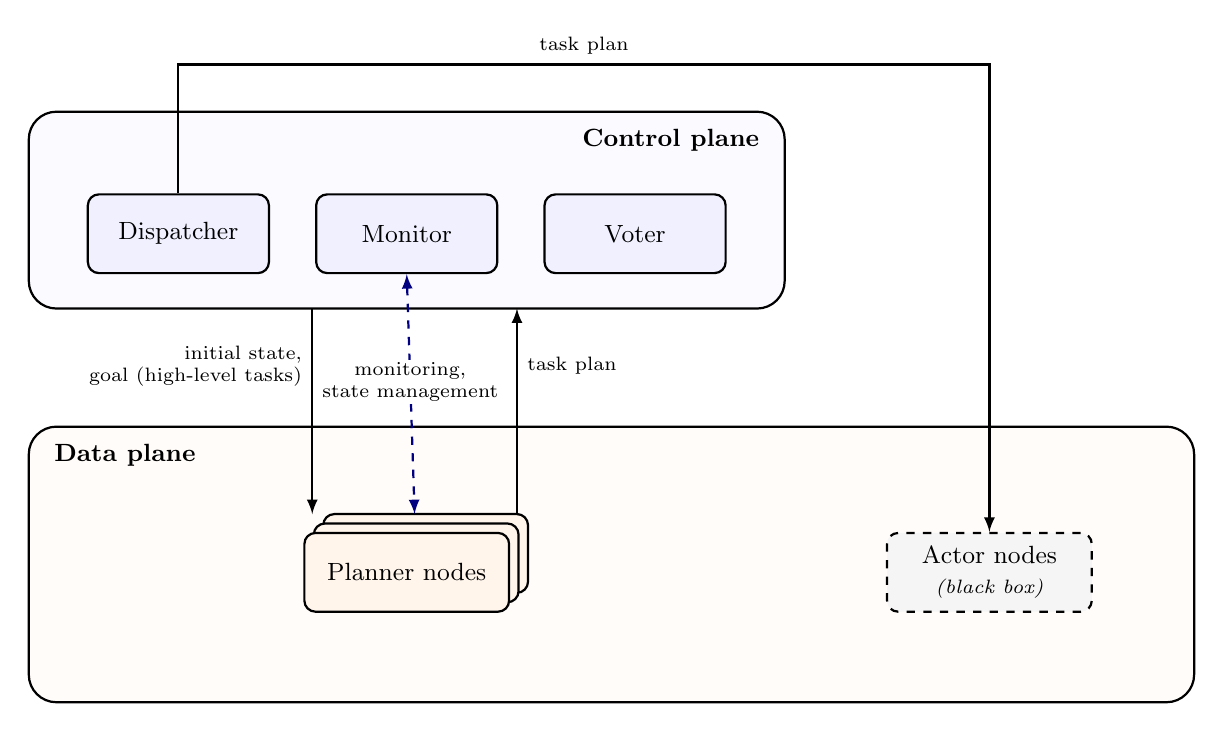
\begin{tikzpicture}[
      >=latex,
      font=\small,
      plane/.style={draw, thick, rounded corners=10pt},
      ctrl/.style ={draw, thick, rounded corners=4pt, fill=blue!6, align=center,
                    minimum width=2.3cm, minimum height=1.0cm},
      data/.style ={draw, thick, rounded corners=4pt, fill=orange!8, align=center,
                    minimum width=2.6cm, minimum height=1.0cm},
      planelbl/.style={font=\small\bfseries, anchor=north west},
      flow/.style ={->, thick},
    ]
    % ---------------- Control plane ----------------
    \draw[plane, fill=blue!2] (0,0) rectangle (9.6,2.5);
    \node[planelbl, anchor=north east] at (9.4,2.4) {Control plane};
    \node[ctrl] (disp) at (1.9,0.95) {Dispatcher};
    \node[ctrl] (mon)  at (4.8,0.95) {Monitor};
    \node[ctrl] (vot)  at (7.7,0.95) {Voter};

    % ---------------- Data plane ----------------
    \draw[plane, fill=orange!2] (0,-5.0) rectangle (14.8,-1.5);
    \node[planelbl] at (0.2,-1.6) {Data plane};

    % Planner nodes (stack = replicated nodes)
    \foreach \d in {0.24,0.12} {
      \node[data] at (4.8+\d,-3.35+\d) {};
    }
    \node[data] (plan) at (4.8,-3.35) {Planner nodes};

    % Actor nodes: single black-box component (not replicated)
    \node[data, dashed, fill=black!4] (act) at (12.2,-3.35) {Actor nodes\\{\scriptsize\itshape (black box)}};

    % ---------------- Interactions ----------------
    % Control plane <-> planner nodes (top of the node stack at y = -2.61)
    \draw[flow] (3.6,0) -- node[left, align=right, font=\scriptsize, pos=0.28]
      {initial state,\\goal (high-level tasks)} (3.6,-2.61);
    \draw[flow] (6.2,-2.61) -- node[right, font=\scriptsize, pos=0.72] {task plan} (6.2,0);

    % Monitor <-> planner nodes: monitoring and state management
    \draw[<->, thick, dashed, blue!50!black] (mon.south) -- node[fill=white, align=center,
      font=\scriptsize, pos=0.45, inner sep=1pt, text=black] {monitoring,\\state management} (4.9,-2.61);

    % Dispatcher -> actor nodes
    \draw[flow] (disp.north) |- node[above, pos=0.75, font=\scriptsize] {task plan}
      (12.2,3.1) -- (act.north);
  \end{tikzpicture}

  \caption[Architecture concept with control and data plane]{%
    Initial architecture concept with control plane and data plane.}
  \label{fig:architecture}
\end{figure}

% Needs only TikZ + the positioning library (already loaded via forest in main.tex)
\begin{figure}[htbp]
  \centering
  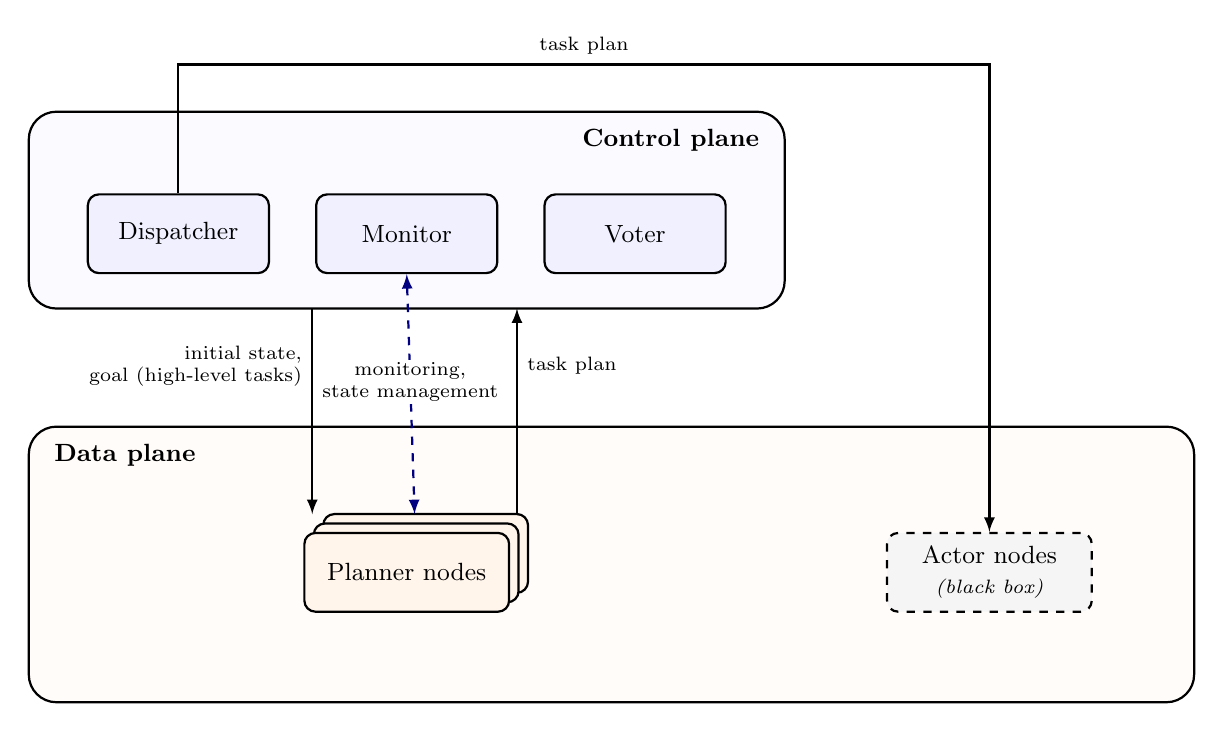
\begin{tikzpicture}[
      >=latex,
      font=\small,
      plane/.style={draw, thick, rounded corners=10pt},
      ctrl/.style ={draw, thick, rounded corners=4pt, fill=blue!6, align=center,
                    minimum width=2.3cm, minimum height=1.0cm},
      data/.style ={draw, thick, rounded corners=4pt, fill=orange!8, align=center,
                    minimum width=2.6cm, minimum height=1.0cm},
      planelbl/.style={font=\small\bfseries, anchor=north west},
      flow/.style ={->, thick},
    ]
    % ---------------- Control plane ----------------
    \draw[plane, fill=blue!2] (0,0) rectangle (9.6,2.5);
    \node[planelbl, anchor=north east] at (9.4,2.4) {Control plane};
    \node[ctrl] (disp) at (1.9,0.95) {Dispatcher};
    \node[ctrl] (mon)  at (4.8,0.95) {Monitor};
    \node[ctrl] (vot)  at (7.7,0.95) {Voter};

    % ---------------- Data plane ----------------
    \draw[plane, fill=orange!2] (0,-5.0) rectangle (14.8,-1.5);
    \node[planelbl] at (0.2,-1.6) {Data plane};

    % Planner nodes (stack = replicated nodes)
    \foreach \d in {0.24,0.12} {
      \node[data] at (4.8+\d,-3.35+\d) {};
    }
    \node[data] (plan) at (4.8,-3.35) {Planner nodes};

    % Actor nodes: single black-box component (not replicated)
    \node[data, dashed, fill=black!4] (act) at (12.2,-3.35) {Actor nodes\\{\scriptsize\itshape (black box)}};

    % ---------------- Interactions ----------------
    % Control plane <-> planner nodes (top of the node stack at y = -2.61)
    \draw[flow] (3.6,0) -- node[left, align=right, font=\scriptsize, pos=0.28]
      {initial state,\\goal (high-level tasks)} (3.6,-2.61);
    \draw[flow] (6.2,-2.61) -- node[right, font=\scriptsize, pos=0.72] {task plan} (6.2,0);

    % Monitor <-> planner nodes: monitoring and state management
    \draw[<->, thick, dashed, blue!50!black] (mon.south) -- node[fill=white, align=center,
      font=\scriptsize, pos=0.45, inner sep=1pt, text=black] {monitoring,\\state management} (4.9,-2.61);

    % Dispatcher -> actor nodes
    \draw[flow] (disp.north) |- node[above, pos=0.75, font=\scriptsize] {task plan}
      (12.2,3.1) -- (act.north);
  \end{tikzpicture}

  \caption[Architecture concept with control and data plane]{%
    Initial architecture concept with control plane and data plane.}
  \label{fig:architecture}
\end{figure}

% Needs only TikZ + the positioning library (already loaded via forest in main.tex)
\begin{figure}[htbp]
  \centering
  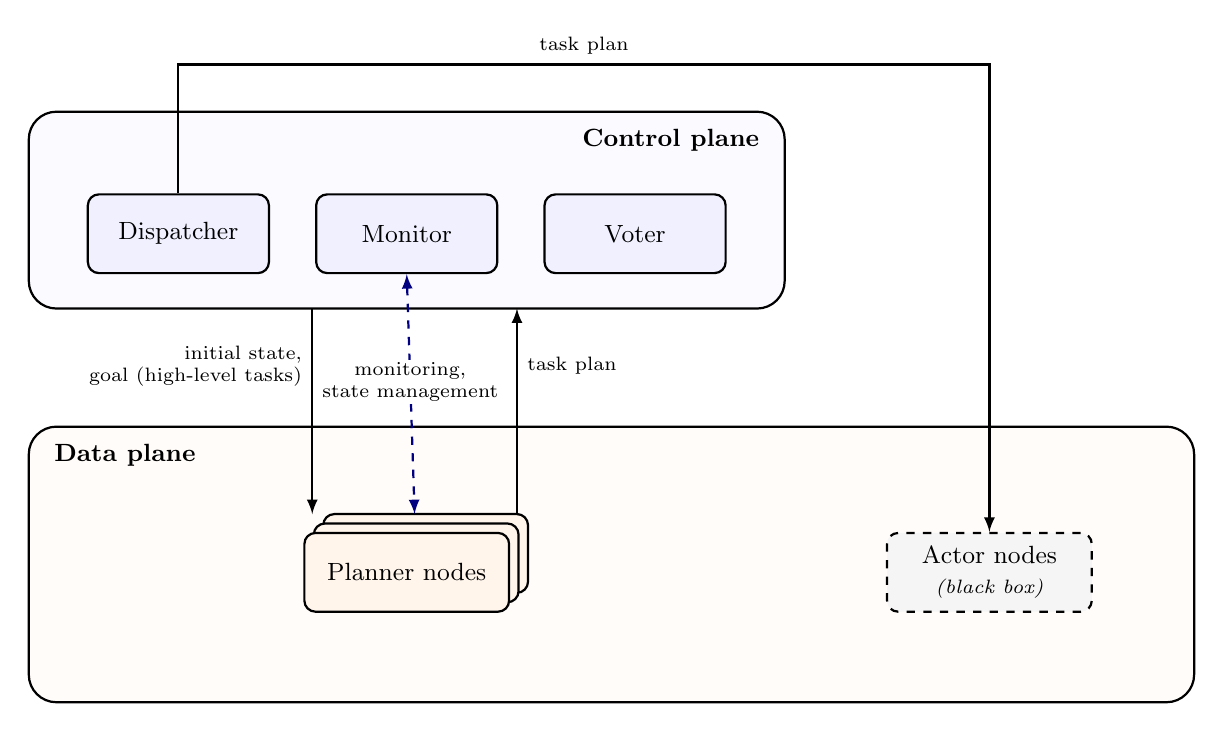
\begin{tikzpicture}[
      >=latex,
      font=\small,
      plane/.style={draw, thick, rounded corners=10pt},
      ctrl/.style ={draw, thick, rounded corners=4pt, fill=blue!6, align=center,
                    minimum width=2.3cm, minimum height=1.0cm},
      data/.style ={draw, thick, rounded corners=4pt, fill=orange!8, align=center,
                    minimum width=2.6cm, minimum height=1.0cm},
      planelbl/.style={font=\small\bfseries, anchor=north west},
      flow/.style ={->, thick},
    ]
    % ---------------- Control plane ----------------
    \draw[plane, fill=blue!2] (0,0) rectangle (9.6,2.5);
    \node[planelbl, anchor=north east] at (9.4,2.4) {Control plane};
    \node[ctrl] (disp) at (1.9,0.95) {Dispatcher};
    \node[ctrl] (mon)  at (4.8,0.95) {Monitor};
    \node[ctrl] (vot)  at (7.7,0.95) {Voter};

    % ---------------- Data plane ----------------
    \draw[plane, fill=orange!2] (0,-5.0) rectangle (14.8,-1.5);
    \node[planelbl] at (0.2,-1.6) {Data plane};

    % Planner nodes (stack = replicated nodes)
    \foreach \d in {0.24,0.12} {
      \node[data] at (4.8+\d,-3.35+\d) {};
    }
    \node[data] (plan) at (4.8,-3.35) {Planner nodes};

    % Actor nodes: single black-box component (not replicated)
    \node[data, dashed, fill=black!4] (act) at (12.2,-3.35) {Actor nodes\\{\scriptsize\itshape (black box)}};

    % ---------------- Interactions ----------------
    % Control plane <-> planner nodes (top of the node stack at y = -2.61)
    \draw[flow] (3.6,0) -- node[left, align=right, font=\scriptsize, pos=0.28]
      {initial state,\\goal (high-level tasks)} (3.6,-2.61);
    \draw[flow] (6.2,-2.61) -- node[right, font=\scriptsize, pos=0.72] {task plan} (6.2,0);

    % Monitor <-> planner nodes: monitoring and state management
    \draw[<->, thick, dashed, blue!50!black] (mon.south) -- node[fill=white, align=center,
      font=\scriptsize, pos=0.45, inner sep=1pt, text=black] {monitoring,\\state management} (4.9,-2.61);

    % Dispatcher -> actor nodes
    \draw[flow] (disp.north) |- node[above, pos=0.75, font=\scriptsize] {task plan}
      (12.2,3.1) -- (act.north);
  \end{tikzpicture}

  \caption[Architecture concept with control and data plane]{%
    Initial architecture concept with control plane and data plane.}
  \label{fig:architecture}
\end{figure}


Necessary components at control plane level for a hierarchical task network include a dispatcher for the initial state and goal, state monitoring (e.g. monitor or observer) of worker nodes and a voter per redundant component.

\section{Components and Functional Assignment}

\subsection{Voter}
During offline development, it is possible to define the task tree (compound task -> subtasks) which would be searched through using DFS. DFS is a deterministic search algorithm and would lead to the same exact search path every time when given the same set of input parameters - in the case of SHOP planners this is the initial world state. What is possible is that tasks are assigned IDs which can be passed with their parameters to a hash function. The voter can match hashes.

Following the use of hashes, two possible designs emerge from this with varying system properties. One hash can be computed with the array of hashes coming from each task plus parameters and pass it to the voter or the voter gets a longer task and compares three arrays of hashes received from each node. The first design would allow for zero overhead in voting because the voter can compute with \(O(1)\) the comparison of three hashes and only checks for an equal match. The drawback here is that this doesn’t allow for any diagnostic visibility. If in a redundant cluster of nodes A, B, C the node C were to fail, the voter can determine that C has failed but cannot see where the error occurred in C.

With the second option of sending the arrays of each node to the voter, the complexity changes to \(O(n)\) with \(n\) number of elements in each array. This would allow the voter to recognize where in the task order an error occurred and in which node. The voter can log this to allow for either real-time diagnosis and error-handling or the same offline. On the point of execution of the tasks, the voter can dispatch tasks which have already been verified while succeeding tasks are still in queue to be verified in the case of long plans. One risk here is if there are succeeding tasks which contain faults that cause the subsequent execution to be halted completely.

If an actuator system has a constraint or requirement that necessitates complete verification, e.g. because of priority level or a critical task that must execute atomically, the method of dispatching verified tasks before all tasks in an array have been verified may be excluded - which is termed for simplicity here as a progressive voter. There is no implication that these implementation designs are mutually exclusive, there can be combinations in one system or two cooperating systems where one uses an atomic voter while the other uses a progressive voter.

Because the voter in this design would only be receiving hashes, it cannot pass the actual task set and their respective parameters to the sub-system or nodes that execute these functions. Further analysis must be done to develop a concept which messages must be exchanged for confirmation of task verification and how the task set is passed to actuators.

While DFS would allow for the same path of search when running identical task trees, there is the case where the ordering of tasks doesn't match for a selected solution task set in the individual nodes. This would occur e.g. in SHOP2 where partial ordering is possible as per \cite{nau_shop2_2003}. The question here is how a voter can resolve this to select one set which is to be passed further to the actuator (systems). One method for this can be by adding a similarity score with a threshold, this method has been extensively researched already and termed as inexact voting \parencite{parhami_voting_1994} where two objects \(x_i\) and \(x_j\) are considered equal if their difference \(d\) fulfills
\[
d(x_i, x_j) \le \epsilon \implies x_i \approx x_j
\]
for a designated threshold \(\epsilon\). If the variation or spread is too far apart, the voter resolves by a best of three match and may reject if this design is extended to compare not only two objects \(x_i\) and \(x_j\), but the total difference \(d(x_{\min}, x_{\max})\). A flaw which is introduced by this would occur when two of the three redundant nodes are equally incorrect, e.g. due to software error or hardware error, and the voter resolves falsely as a correct solution because the threshold bound constraint is still fulfilled.
A design concern would be whether the voter comparison can still work if the order in which hashes are received can vary because of varying orders. This can be solved by switching the data structure in which the voter receives the task sets and use a dictionary instead. Earlier an array was described as a possibility, which is still beneficial since arrays are a smaller data structure which is ideal for data transmission to reduce the data bus occupancy necessary for communication between individual components.
The data structure used for communication has no direct design constraint on what other data structure it can be refactored into when processed in the voter itself. If it's more ideal for parsing in the voter, this can be considered for an unordered comparison.
Since the scope is restricted to not use any thresholds in voting, the original SHOP planner excludes this by design because no partial ordering is used and no similarity score would be required to compensate for non-identical orders. Here the voter need not use any similarity score or any response for a scenario of equally incorrect solutions which can 'trick' the voter.

With the voter's constraint on how much information it receives (hashes) or can return for the individual nodes (positive or negative), it only takes the role of an arbiter / referee. This splits the responsibilities in the architecture into a data plane and a control plane. The control plane logic can be traced to other domains using decentralized management like in SDNs or orchestration methods in cloud computing, e.g. Kubernetes clusters.

\subsection{Monitor}

The monitor can be designed in multiple ways. One possibility is to use a polling approach where the monitor periodically sends a message to the planner nodes, which then send a response. In this case, the monitor tracks state of response time to determine a timeout. Monitoring of actuator nodes will be excluded to restrict scope focus on planner node redundancy, this means actuators will be viewed as a black box component.
The second possible design is to have all planner nodes periodically send the monitor their heartbeat messages without prior prompting from the monitor, this would be a push-style monitor. This reduces message count which is beneficial to real systems where data bus bandwidths are typically low and only necessary information is exchanged. The monitor then operates on a primary read functionality by tracking state of messages received with a defined timeout duration based on frequency of heartbeat messages. For a frequency \(f\), the timeout can be calculated as multiples \(n\) of the period \(T = \frac{1}{f}\) and \(T_{\text{timeout}} = n \cdot \frac{1}{f} = n \cdot T\).
The frequency of the heartbeat messages is strictly constrained at maximum by frequency of transmission of the bus system being used in a real avionic system. Depending on how critical a redundant component is, this must be determined on a case-by-case basis to allocate properly the required bandwidth and occupancy rate per time on a bus.

As the complementary function, the monitor must have a response for a watchdog timer expiration. If designed as a per-redundant-node monitor, this can be used to detect the unresponsive node and send a signal to restart specifically the affected node. This isn't the only possible design here, there are many other variations possible such as signaling the entire cluster that a node is currently unavailable (and restarting or other error-handling), which can be useful for larger systems where other dependent sub-systems would need to use their own fallback mechanism in a case of node failure.

\cite{bonna_triple_2019} describe a mechanism where the voter handles monitoring and, upon receipt of a differing output, assumes a fault in such processor. Here the error-handling is done by sending a signal to the control device to compensate for said fault, in the case of \cite{bonna_triple_2019} this is done with runtime reconfigurable processors (RTRP). This method would be applicable for hardware faults. Another approach has been developed to compensate for hardware faults by dynamically switching to Temporal Software Redundancy (TSR) \parencite{hamilton_adaptive-hybrid_2019}. A controller monitors the system for consecutive errors in execution to transition between TMR and a lower-power TSR. The difference here is not only in how the system can handle failures, but also which implications it has on resource utilization. TMR requires three physical processors operating concurrently alongside a hardware majority voter while TSR runs on a single processor, thus requiring less power. In avionic systems, this can be useful when hardware failures compromise power delivery to the redundant cluster, where power distribution may be constrained.

\subsection{State synchronization and Dispatcher}

Both of these approaches need to account for state synchronization in the software and hardware for the new system state when error-handling has been executed successfully. For methods using TMR and TSR and the former with RTRP, this has been done through memory \parencite{bonna_triple_2019, hamilton_adaptive-hybrid_2019}. The choice here depends on what production cost is viable for the number of hardware components to be used in a redundant cluster. Another factor is how critical a function is, since RTRP also makes use of overriding less critical applications when a processor of a higher priority function incurs an error during execution \parencite{bonna_triple_2019}. This means systems to which more cost is allocated for the number of processors, and other hardware components (e.g. memory, controllers, etc.), can still utilize non-primary hardware which allows for a better utilization of all resources, rather than keeping an excess of hardware resources on idle.

As a consequence of state synchronization due to error-handling, an HTN-cluster would need to have checkpoints defined where a re-synchronization is possible to reduce the number of states for which the system must have recovery routines defined. This state synchronization is not the same type which a dispatcher would be handling because the main question in this case is how the system can compensate for synchronization when errors occur. Synchronization mechanisms described later in the dispatcher design are defined for intended behavior of the redundant cluster. Therefore the role of the monitor is to respond or initiate a recovery routine when unintended behavior occurs.

One common problem that occurs in distributed systems is delay and variation in timing between individual components. This has already been extensively researched \parencite{lamport_time_1978, steen_distributed_2025}. In the context of a TMR-node cluster used in the concept of this architecture, the same applies in variation of time required for processing, calculation of a plan and outbound transmission to a voter for the software side. As for variations and delays introduced by real electronic systems, the number of possible points where delays occur only increases, i.e. bus frequency, transmission frequency by sender(s), electromagnetically induced variations, jitter, propagation time, etc.\\
Exploring the entire solution space here would be too large and thus needs to be bound by an acceptable frame within which questions can be addressed on the theoretical side and a subsequent connection of the possible solution space with real-world implications in safety-critical systems and their limitations. The scope is defined to address critical points which can be handled by the dispatcher. The first critical point is receipt of input data, then the verification by a voter and thirdly the transmission of the final task plan to the actuator system(s). If the scope were simplified further to only address the last critical point which was just mentioned (transmission to the actuator systems), a strict limitation would be introduced in the capabilities of the dispatcher when applied to real avionic systems. To reduce the number of hardware components, there cannot be a central server or an equivalent to monitor other subsystems which this architecture is dependent on. This functionality can be added to the dispatcher to verify if these subsystems are providing data correctly. In a simple form this can be designed as a read-only check where the dispatcher verifies if it is receiving a message by each of its required sources, which can be a heartbeat message or only the input data which is to be forwarded to the worker nodes. Another addition can be connected to the protocol TCP where an explicit ACK is sent to the sender. This is also found under MIL-STD-1553C, as receipt and validation of messages are confirmed by using the Status Word. Both acknowledgements are required on two different levels since the former is as defined by the ISO/OSI seven-layer model at the transport layer while the latter is relevant for the physical and data link layer.

To discern the function which an acknowledgement would serve here, it isn't used here to determine whether communication was successful, since the architecture defines guaranteed message delivery. Instead it can be used here to confirm system liveness to external systems. In safety-critical systems, the bus design may be separated as an intra-system bus and another design for an inter-system bus. The inter-system bus may be shared among several sub-systems, meaning bus occupancy rate must be reduced by each individual system to mitigate failures or errors in communication when messaging traffic is higher. This would exclude the design option to use heartbeat messages between subsystems and require a method that uses a lower message frequency, e.g. acknowledgements.
Upon receipt of required input data, the dispatcher would send it concurrently to a redundant node cluster of worker nodes. This would allow synchronization for the starting time when the worker nodes calculate a task plan.

The second critical point for the dispatcher is when a voter has successfully verified a task plan. A successful verification is defined as one completed routine of a voter having verified a list of tasks without cancelling the routine until all tasks have been verified. In this architecture, the dispatcher wouldn't have any direct communication with a voter, it would only receive the task sets from the node cluster.
\\
Upon receipt of task plans from the nodes which were verified as correct by the voter, the dispatcher may select arbitrarily (e.g. randomized) or based on defined criteria which plan it may select to send to the actuator(s).


\section{Proof of Concept}
% Explain the implementation, tools, and relevant design details.